\documentclass[12pt]{article}
\usepackage[a4paper, margin=1in]{geometry}
\usepackage{xeCJK}
\usepackage{amsmath}
\usepackage{graphicx}
\usepackage{natbib}
\usepackage{booktabs}
\usepackage{caption}
\usepackage{hyperref}
\usepackage{listings}
\usepackage{graphicx}
\usepackage{pythonhighlight}
\setCJKmainfont{SimSun} % 使用宋体


% 设置页面格式
\linespread{1.5}
\title{冷热电联供系统综合评价方法研究与实现}
\author{唐玮嘉 \\ 学号: 2023428020130 \\ 学校: 东莞理工学院 \\ 专业: 能源与动力工程}
\date{\today}

\begin{document}

\maketitle

\begin{abstract}
冷热电联供(CCHP)系统因其高效、节能和环保的特性,广泛应用于分布式能源领域。本文基于混合多层次灰色关联综合评价方法,对五种CCHP系统方案进行综合评价,综合考虑经济性、环境性、社会性、性能和噪声等指标。通过层次分析法(AHP)计算权重,模糊隶属函数量化定性指标,灰色关联分析评估方案优劣,并使用Python实现算法。结果表明,方案C在综合性能上表现最佳。本文总结了方法实现过程,验证了算法的有效性,并为CCHP系统优化设计提供了参考。
\end{abstract}

\section{引言}
冷热电联供(Combined Cooling, Heating, and Power, CCHP)系统通过集成发电、制冷和供热功能,实现能源梯级利用,具有高效节能和低排放的优势 \citep{cho2014combined}。然而,CCHP系统的设计需综合考虑经济性、环境性、社会性等多方面因素,评价方法的选择直接影响方案优化的科学性。本次作业基于混合多层次灰色关联综合评价方法,对五种CCHP系统方案进行评价,旨在验证方法的有效性和实现过程。

\section{评价方法}

\subsection{方法框架}
本文采用混合多层次灰色关联综合评价方法,结合层次分析法(AHP)、模糊量化、数据标准化和灰色关联分析。主要步骤包括:
\begin{enumerate}
    \item 构建评价指标体系,包含经济性、环境性、社会性、性能和噪声五大类,共12个子指标。
    \item 使用AHP计算一级和二级指标权重。
    \item 通过模糊隶属函数量化社会性定性指标。
    \item 对指标数据进行标准化处理,区分正指标和逆指标。
    \item 基于灰色关联分析计算各方案的综合关联度,排序得出最优方案。
\end{enumerate}

\subsection{关键算法}

\subsubsection{层次分析法(AHP)}
AHP通过构造判断矩阵,计算各指标的相对重要性权重。本文采用行和归一化法:
\[
w_i = \frac{\sum_{j=1}^n a_{ij}}{\sum_{i=1}^n \sum_{j=1}^n a_{ij}}
\]
其中,$a_{ij}$为判断矩阵元素,$w_i$为第$i$个指标的权重。

\subsubsection{模糊量化}
社会性指标(如技术先进性)为定性指标,采用分段模糊隶属函数量化:
\[
f(x) = \begin{cases} 
\frac{1}{1 + 1.1086 (x - 0.8942)^{-2}}, & 1 \leq x \leq 3 \\
0.3915 \ln x + 0.3699, & 3 < x \leq 5 
\end{cases}
\]

\subsubsection{数据标准化}
为消除量纲影响,对正指标和逆指标分别标准化:
\[
z_i(k) = \frac{x_i(k) - \min x_i(k)}{\max x_i(k) - \min x_i(k)} \quad (\text{正指标})
\]
\[
z_i(k) = \frac{\max x_i(k) - x_i(k)}{\max x_i(k) - \min x_i(k)} \quad (\text{逆指标})
\]

\subsubsection{灰色关联分析}
以全1向量为参考序列,计算关联系数:
\[
\xi_i(k) = \frac{\min_i \min_k |\Delta_i(k)| + \rho \max_i \max_k |\Delta_i(k)|}{|\Delta_i(k)| + \rho \max_i \max_k |\Delta_i(k)|}
\]
综合关联度为:
\[
r_i = \sum_{k=1}^{12} w_k \cdot \xi_i(k)
\]
其中,$\rho=0.5$为分辨系数。

\section{算法实现}
算法使用Python实现,核心模块包括:
\begin{itemize}
    \item \textbf{数据输入}:定义5个方案的12个指标数据,指标性质(正/逆)明确。
    \item \textbf{权重计算}:实现AHP权重计算函数,处理一级和二级判断矩阵。
    \item \textbf{模糊量化}:对社会性指标应用模糊隶属函数。
    \item \textbf{标准化}:实现正逆指标的标准化处理。
    \item \textbf{灰色关联分析}:计算关联系数和综合关联度。
    \item \textbf{结果可视化}:使用Matplotlib绘制柱状图,展示各方案的关联度。
\end{itemize}

代码运行环境为Python 3.11,依赖NumPy、Pandas和Matplotlib库。关键代码片段如下:
\begin{python}[caption=关键算法实现]
def fuzzy_quantization(data):
    def _f(x):
        if x >= 3:
            return 0.3915 * np.log(x) + 0.3699
        else:
            return 1 / (1 + 1.1086 / ((x - 0.8942)**2 + 1e-9))
    return np.vectorize(_f)(data)

def grey_relation(norm_data, weights, rho=0.5):
    ideal = np.ones(norm_data.shape[1])
    delta = np.abs(norm_data - ideal)
    min_delta = np.min(delta)
    max_delta = np.max(delta)
    xi = (min_delta + rho*max_delta) / (delta + rho*max_delta)
    return np.dot(xi, weights)
\end{python}

\section{结果与讨论}

\subsection{评价结果}
五种方案的灰色关联度如表~\ref{tab:results}所示,方案E的关联度最高(0.7972),表明其综合性能最优。

\begin{table}[ht]
\centering
\caption{各方案灰色关联度排序}
\label{tab:results}
\begin{tabular}{lc}
\toprule
方案 & 灰色关联度 \\
\midrule
方案E & 0.7972 \\
方案C & 0.6569 \\
方案A & 0.6062 \\
方案B & 0.5792 \\
方案D & 0.5457 \\
\bottomrule
\end{tabular}
\end{table}

\subsection{结果可视化}
图~\ref{fig:bar}展示了各方案的灰色关联度柱状图,直观反映了方案E的优越性。

\begin{figure}[ht]
\centering
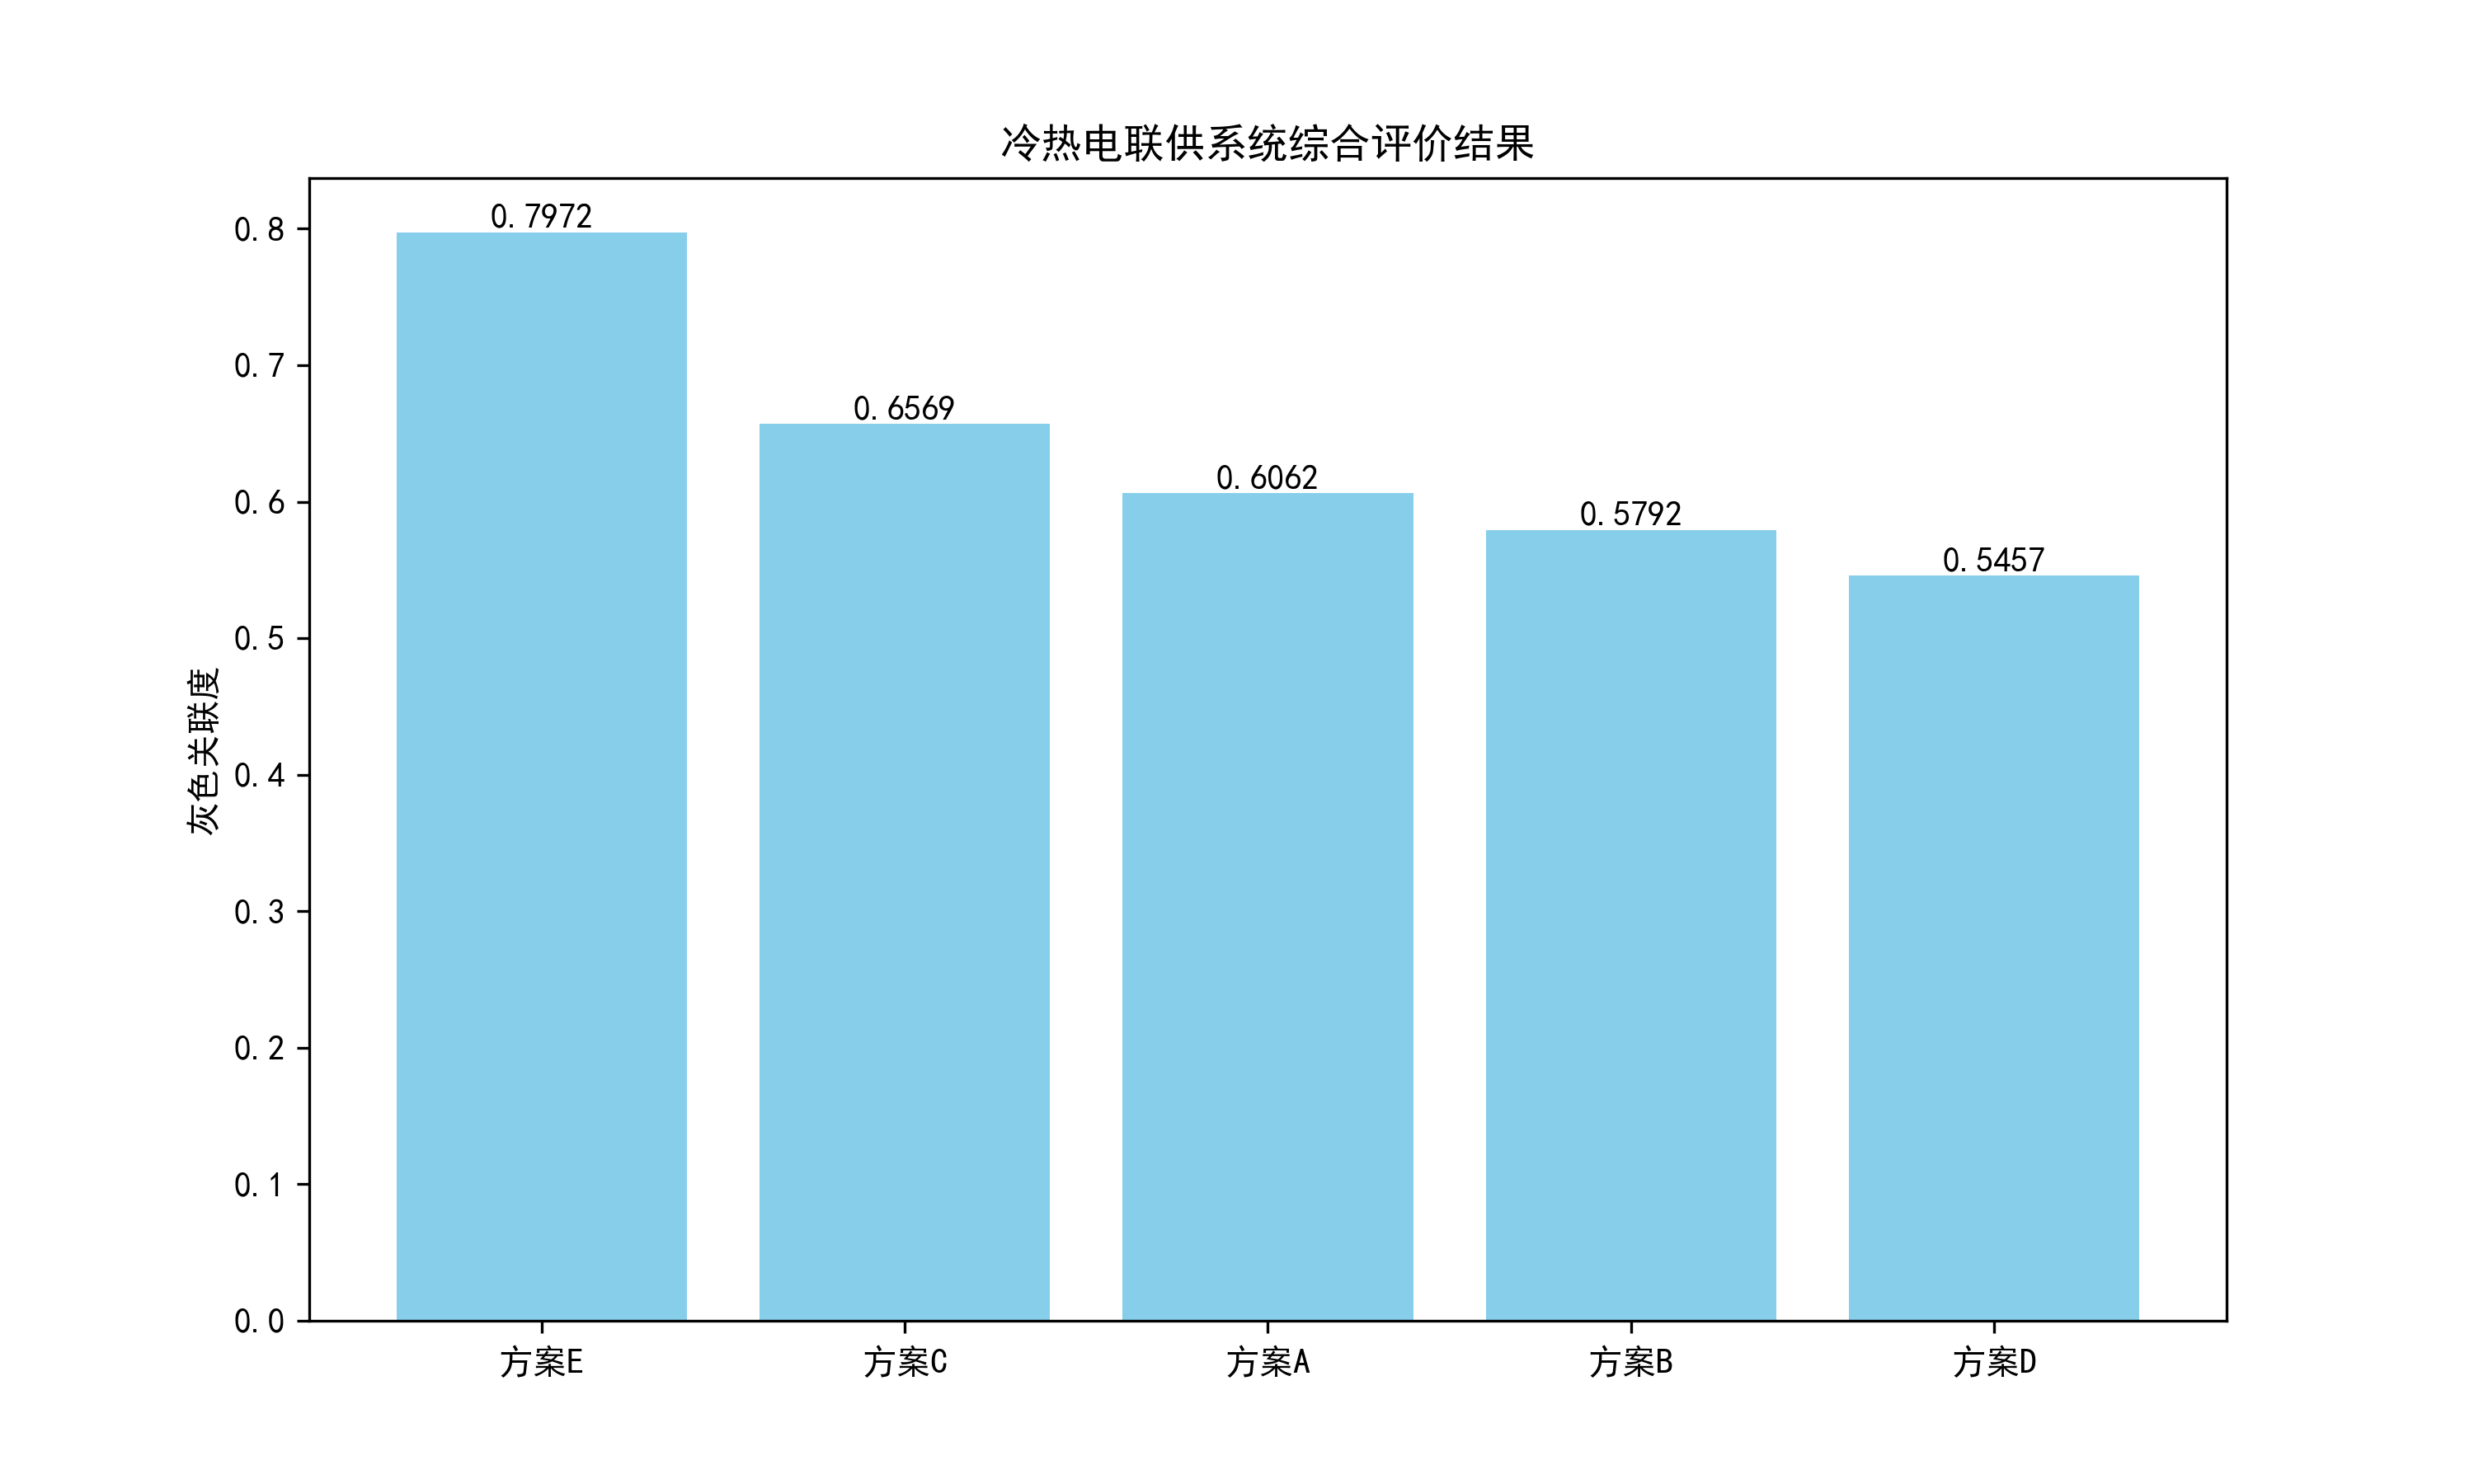
\includegraphics[width=0.8\textwidth]{../code/fig1/综合评价结果.png}
\caption{冷热电联供系统综合评价结果}
\label{fig:bar}
\end{figure}

\subsection{讨论}
方案C在经济性和环境性指标上表现均衡,社会性指标得分较高,噪声和性能指标适中,因而综合评价最优。方案D因经济性指标(如初始投资)较高,关联度最低。结果表明,混合多层次灰色关联方法能有效综合多维度指标,适合CCHP系统评价。

\section{结论}
本文通过混合多层次灰色关联综合评价方法,成功对五种CCHP系统方案进行了评价,验证了方法的科学性和可行性。Python实现高效完成了权重计算、数据处理和结果分析,方案C被确认为最优方案。未来可进一步引入一致性检验和敏感性分析,提升方法的鲁棒性。本作业为CCHP系统优化设计提供了实践参考。

\bibliographystyle{plain}
\bibliography{references}

\section{附录}
% python代码

\begin{python}[language=Python, caption= 全部代码]

import os
import numpy as np
import pandas as pd
import matplotlib.pyplot as plt
from matplotlib.font_manager import FontProperties

# 支持中文显示
plt.rcParams['font.sans-serif'] = ['SimHei']
plt.rcParams['axes.unicode_minus'] = False


dir = 'fig1'
if not os.path.exists(dir):
    os.makedirs(dir)

# ===================== 核心算法模块 =====================
def ahp_weight(matrix):
    """层次分析法权重计算(行和归一化法)"""
    row_sum = np.sum(matrix, axis=1)
    weights = row_sum / np.sum(row_sum)
    return weights

def fuzzy_quantization(data):
    """模糊隶属函数量化(处理定性指标)"""
    def _f(x):
        if x >= 3:
            return 0.3915 * np.log(x) + 0.3699
        else:
            denominator = (x - 0.8942) ** 2 + 1e-9
            return 1 / (1 + 1.1086 / denominator)
    return np.vectorize(_f)(data)

def normalize(data, types):
    """指标标准化处理"""
    normalized = np.zeros_like(data, dtype=float)
    for col in range(data.shape[1]):
        min_val = np.min(data[:, col])
        max_val = np.max(data[:, col])
        if types[col] == 1:  # 正指标
            normalized[:, col] = (data[:, col] - min_val) / (max_val - min_val + 1e-9)
        else:  # 逆指标
            normalized[:, col] = (max_val - data[:, col]) / (max_val - min_val + 1e-9)
    return normalized

def grey_relation(norm_data, weights, rho=0.5):
    """灰色关联度计算"""
    ideal = np.ones(norm_data.shape[1])
    delta = np.abs(norm_data - ideal)
    min_delta = np.min(delta)
    max_delta = np.max(delta)
    
    # 关联系数矩阵
    xi = (min_delta + rho*max_delta) / (delta + rho*max_delta)
    
    # 综合关联度
    return np.dot(xi, weights)

# ===================== 主程序 =====================
def main():
    # ------------ 数据准备 ------------
    # 每个方案包含12个指标的完整数据(不要分割成子列表)
    raw_data = np.array([
        # 方案A: [经济性4, 环境性3, 社会性3, 性能1, 噪声1]
        [535000, 6.42, 480137, 52582, 0.23, 0.45, 400, 0.8, 0.8, 0.6, 1.969, 65],
        # 方案B
        [680000, 6.63, 481374, 28108, 0.223, 0.6, 589, 0.8, 0.8, 0.6, 1.855, 65],
        # 方案C
        [504568, 4.86, 387851, 546633, 0.7, 0.8, 430, 0.6, 0.6, 0.6, 1.594, 80],
        # 方案D 
        [1580000, 8.8, 530131, -403086, 0.007, 0.001, 362, 0.934, 0.934, 0.8, 1.4, 60],
        # 方案E
        [290000, 6.73, 197179, 32136, 3.2, 4, 700, 0.4, 0.4, 0.934, 13.3, 56]
    ])  # shape (5,12) 已确认

    # 指标性质 (0:逆指标,1:正指标)
    index_types = [
        0,0,0,1,   # 经济性(4)
        0,0,0,     # 环境性(3)
        1,1,1,     # 社会性(3)
        0,0        # 性能,噪声(2)
    ]

    # ------------ 权重计算 ------------
    # 一级指标判断矩阵(经济性F1、环境性F2、社会性F3、性能F4、噪声F5)
    L1_matrix = np.array([
        [1, 7, 4, 5, 3],
        [1/7, 1, 1/4, 1/3, 1/5],
        [1/4, 4, 1, 2, 1/3],
        [1/5, 3, 1/2, 1, 1/4],
        [1/3, 5, 3, 4, 1]
    ])
    L1_weights = ahp_weight(L1_matrix)

    # 二级指标权重
    F1_matrix = np.array([  # 经济性
        [1, 3, 5, 7],
        [1/3, 1, 6, 1/4],
        [1/5, 1/6, 1, 1/3],
        [1/7, 4, 3, 1]
    ])
    F1_weights = ahp_weight(F1_matrix) * L1_weights[0]

    F2_matrix = np.array([  # 环境性
        [1, 6, 4],
        [1/6, 1, 1/3],
        [1/4, 3, 1]
    ])
    F2_weights = ahp_weight(F2_matrix) * L1_weights[1]

    F3_matrix = np.array([  # 社会性
        [1, 1/3, 5],
        [3, 1, 7],
        [1/5, 1/7, 1]
    ])
    F3_weights = ahp_weight(F3_matrix) * L1_weights[2]

    # 性能F4和噪声F5作为一级指标直接继承权重
    F4_weights = np.array([L1_weights[3]])
    F5_weights = np.array([L1_weights[4]])

    # 合成总权重
    total_weights = np.concatenate([F1_weights, F2_weights, F3_weights, F4_weights, F5_weights])

    # ------------ 数据处理 ------------
    # 定性指标模糊量化(社会性)
    raw_data[:, 7:10] = fuzzy_quantization(raw_data[:, 7:10])

    # 数据标准化
    norm_data = normalize(raw_data, index_types)

    # ------------ 灰色关联分析 ------------
    grey_scores = grey_relation(norm_data, total_weights)

    # ------------ 结果展示 ------------
    results = pd.DataFrame({
        '方案': ['方案A', '方案B', '方案C', '方案D', '方案E'],
        '灰色关联度': grey_scores
    }).sort_values('灰色关联度', ascending=False)

    print("综合评价结果排序:")
    print(results)

    # 可视化
    plt.figure(figsize=(10, 6))
    bars = plt.bar(results['方案'], results['灰色关联度'], color='skyblue')
    plt.title('冷热电联供系统综合评价结果')
    plt.ylabel('灰色关联度')
    for bar in bars:
        yval = bar.get_height()
        plt.text(bar.get_x() + bar.get_width()/2, yval, f'{yval:.4f}', 
                va='bottom', ha='center')
    plt.savefig('fig1/综合评价结果.png', dpi=300)
    plt.show()

if __name__ == "__main__":
    main()

\end{python}


\end{document}

